%\iffalse
\let\negmedspace\undefined
\let\negthickspace\undefined
\documentclass[journal,12pt,twocolumn]{IEEEtran}
\usepackage{cite}
\usepackage{amsmath,amssymb,amsfonts,amsthm}
\usepackage{algorithmic}
\usepackage{graphicx}
\usepackage{textcomp}
\usepackage{xcolor}
\usepackage{txfonts}
\usepackage{listings}
\usepackage{enumitem}
\usepackage{mathtools}
\usepackage{gensymb}
\usepackage{comment}
\usepackage[breaklinks=true]{hyperref}
\usepackage{tkz-euclide} 
\usepackage{listings}
\usepackage{gvv}                                        
\def\inputGnumericTable{}                                 
\usepackage[latin1]{inputenc}                                
\usepackage{color}                                            
\usepackage{array}                                            
\usepackage{longtable}                                       
\usepackage{calc}                                             
\usepackage{multirow}                                         
\usepackage{hhline}                                           
\usepackage{ifthen}                                           
\usepackage{lscape}
\newtheorem{theorem}{Theorem}[section]
\newtheorem{problem}{Problem}
\newtheorem{proposition}{Proposition}[section]
\newtheorem{lemma}{Lemma}[section]
\newtheorem{corollary}[theorem]{Corollary}
\newtheorem{example}{Example}[section]
\newtheorem{definition}[problem]{Definition}
\newcommand{\BEQA}{\begin{eqnarray}}
\newcommand{\EEQA}{\end{eqnarray}}
\newcommand{\define}{\stackrel{\triangle}{=}}
\theoremstyle{remark}
\newtheorem{rem}{Remark}
\begin{document}

\bibliographystyle{IEEEtran}
\vspace{3cm}

\title{DISCRETE}
\author{EE23BTECH11006 - Ameen Aazam$^{*}$% <-this % stops a space
}
\maketitle
\newpage
\bigskip

\renewcommand{\thefigure}{\theenumi}
\renewcommand{\thetable}{\theenumi}

\vspace{3cm}
\textbf{Question :}
Find the sum of the following APs:
\begin{enumerate}[label=(\alph*)]
\item $2, 7, 12, \ldots$ to $10$ terms.
\item $-37, -33, -29, \ldots$ to $12$ terms.
\item $0.6, 1.7, 2.8, \ldots$ to $100$ terms.
\item $\frac{1}{15}, \frac{1}{12}, \frac{1}{10}, \ldots$ to $11$ terms.
\end{enumerate}
\solution
%\fi
\begin{table}[htbp]
    \centering
    \begin{tabular}{|c|c|c|} \hline
      \textbf{Input Parameters} & \textbf{Values} & \textbf{Description} \\ \hline
      $n$ & & Independent Variable \\ \hline
      $a$ & & First term of $1^{st}$ G.P. \\ \hline
      $r$ & & Common ratio of $1^{st}$ G.P. \\ \hline
      $x_1\brak{n}$ & $x_1\brak{n}=ar^nu\brak{n}$& General term of $1^{st}$ G.P. \\ \hline
      $X_1\brak{z}$ & & z-Transform of $1^{st}$ G.P. \\ \hline
      $A$ & & First term of $2^{nd}$ G.P. \\ \hline
      $R$ & & Common ratio of $2^{nd}$ G.P. \\ \hline
      $x_2\brak{n}$ & $x_1\brak{n}=AR^nu\brak{n}$& General term of $2^{nd}$ G.P. \\ \hline
      $X_2\brak{z}$ & & z-Transform of $2^{nd}$ G.P. \\ \hline
    \end{tabular}
    \vspace{3pt}
    \caption{Parameters}
    \label{tab:11.9.3.20.tab}
\end{table}

From \eqref{eq:abc}, we get the sum to $n$ terms,
\begin{align}
    y(n)=\frac{(n+1)}{2}\cbrak{2x(0)+nd}u(n)
\end{align}
Now taking the Z-transform we have,
\begin{align}
    Y(z)=\frac{x(0)}{(1-z^{-1})^2}+\frac{dz^{-1}}{(1-z^{-1})^3}
\end{align}
\begin{enumerate}[label=(\alph*)]
    \item \begin{align}
        &x(0)=2 \\
        &d=5 \\
        \implies &y(9)=245
    \end{align}
    \begin{figure}[h!]
        \centering
        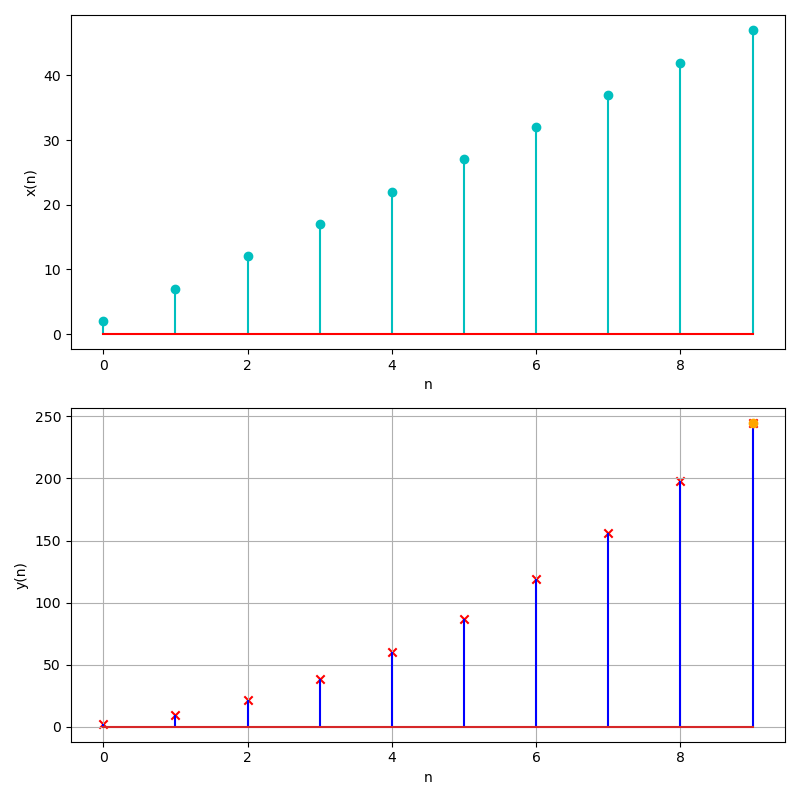
\includegraphics[width=0.9\columnwidth]{figs/plt1.png}
        \caption{$1st$ AP}
    \end{figure}
    \item \begin{align}
        &x(0)=-37 \\
        &d=4 \\
        \implies &y(11)=-180
    \end{align}
    \begin{figure}[h!]
        \centering
        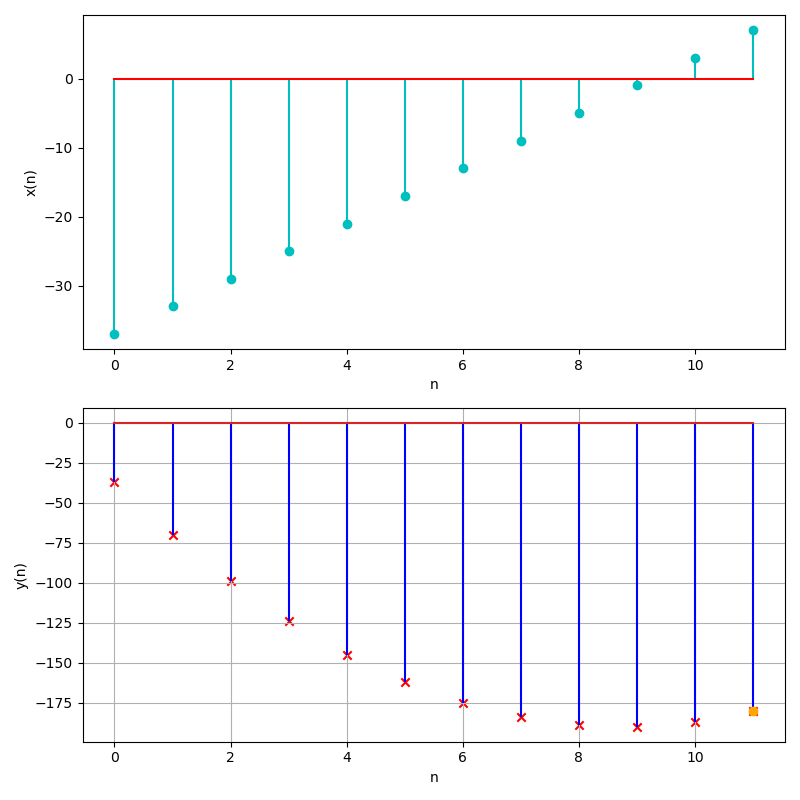
\includegraphics[width=0.9\columnwidth]{figs/plt2.png}
        \caption{$2nd$ AP}
    \end{figure}
    \item \begin{align}
        &x(0)=0.6 \\
        &d=1.1 \\
        \implies &y(99)=5505
    \end{align}
    \begin{figure}[h!]
        \centering
        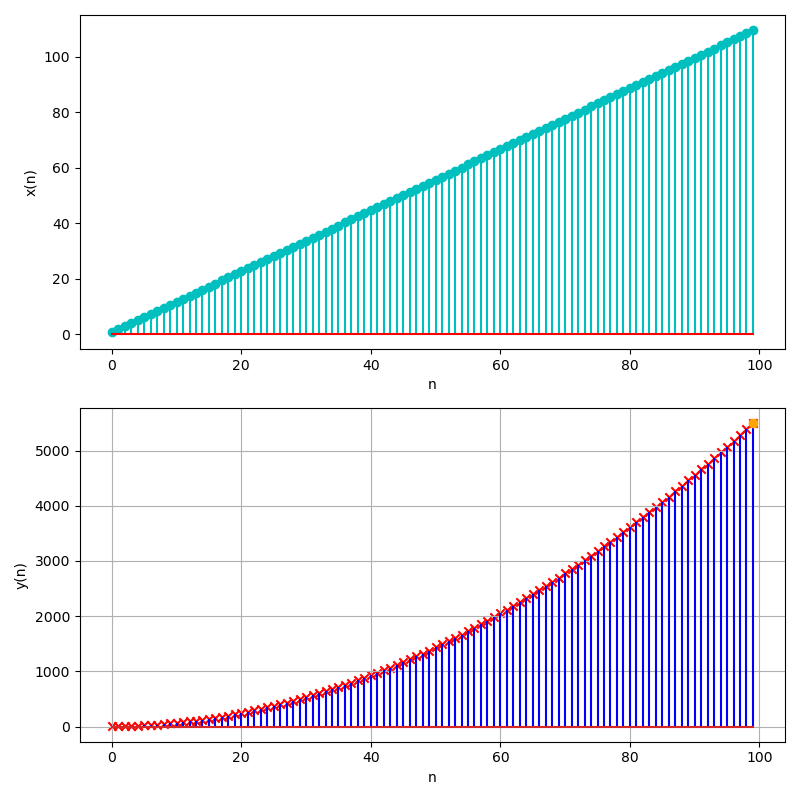
\includegraphics[width=0.9\columnwidth]{figs/plt3.png}
        \caption{$3rd$ AP}
    \end{figure}
    \item \begin{align}
        &x(0)=\frac{1}{15} \\
        &d=\frac{1}{60} \\
        \implies &y(10)=1.65
    \end{align}
    \begin{figure}[h!]
        \centering
        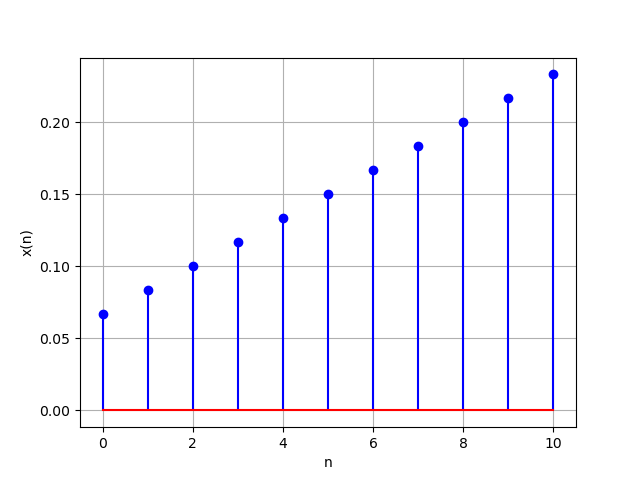
\includegraphics[width=0.9\columnwidth]{figs/plt4.png}
        \caption{$4th$ AP}
    \end{figure}
\end{enumerate}

\end{document}

